\subsection{Lokalen - FR3}

%Lokaal detailformulier toevoegen  
\subsubsection{Lokaal detailformulier toevoegen} 
\noindent\begin{table}[H]
            \begin{tabular}{l | p{10cm}}
                \textbf{ID:} & FR3.1 \\ \hline
                \textbf{TITEL:} & Lokaal detailformulier toevoegen\\ \hline
                \textbf{PRIORITEIT:} &  Hoog \\ \hline
                \textbf{PREREQUISITIES:} & \\ \hline
                \textbf{TOEGANG:} & Programmabeheerder \\ \hline
                \textbf{BESCHRIJVING:} & De Programmabeheerder moet in staat zijn om lokalen toe te voegen aan de database zodat de scheduler die kan gebruiken in zijn planning. Lokalen hebben een ID nummer van de vorm G.V.L (met G = gebouw, V = verdieping en L = lokaal) en hebben ook bepaalde faciliteiten (beamer, overheadprojector...) een maximaal aantal plaatsen, \\ 
            \end{tabular}\\
            \caption{FR3.1 -Lokaal detailformulier toevoegen}
            \label{tab:FR3.1 - Lokaal detailformulier toevoegen}
        \end{table}

\textbf{Stappenplan:}
\begin{enumerate}
\item De programmabeheerder ziet zijn beginscherm op zijn webbrowser. Hier ziet hij de optie "lokalen".
\item De programmabeheerder klikt hierop en wordt doorverwezen naar een nieuwe pagina waar hij de optie ziet om lokalen toe te voegen.
\item De programmabeheerder klikt op deze optie en wordt doorverwezen naar een nieuwe pagina met een formulier om de nodige gegevens van het lokaal in te vullen (zie figuur \ref{fig:CalZone New Classroom}).
\item De programmabeheerder vult deze gegevens correct in en ziet een knop met de naam "Lokaal toevoegen".
\item De programmabeheerder klikt op deze knop en het lokaal wordt toegevoegd in de database en dus ook in het systeem.
\end{enumerate}

\begin{center}
\begin{figure}[H]
\caption{CalZone New Classroom}
\centerline{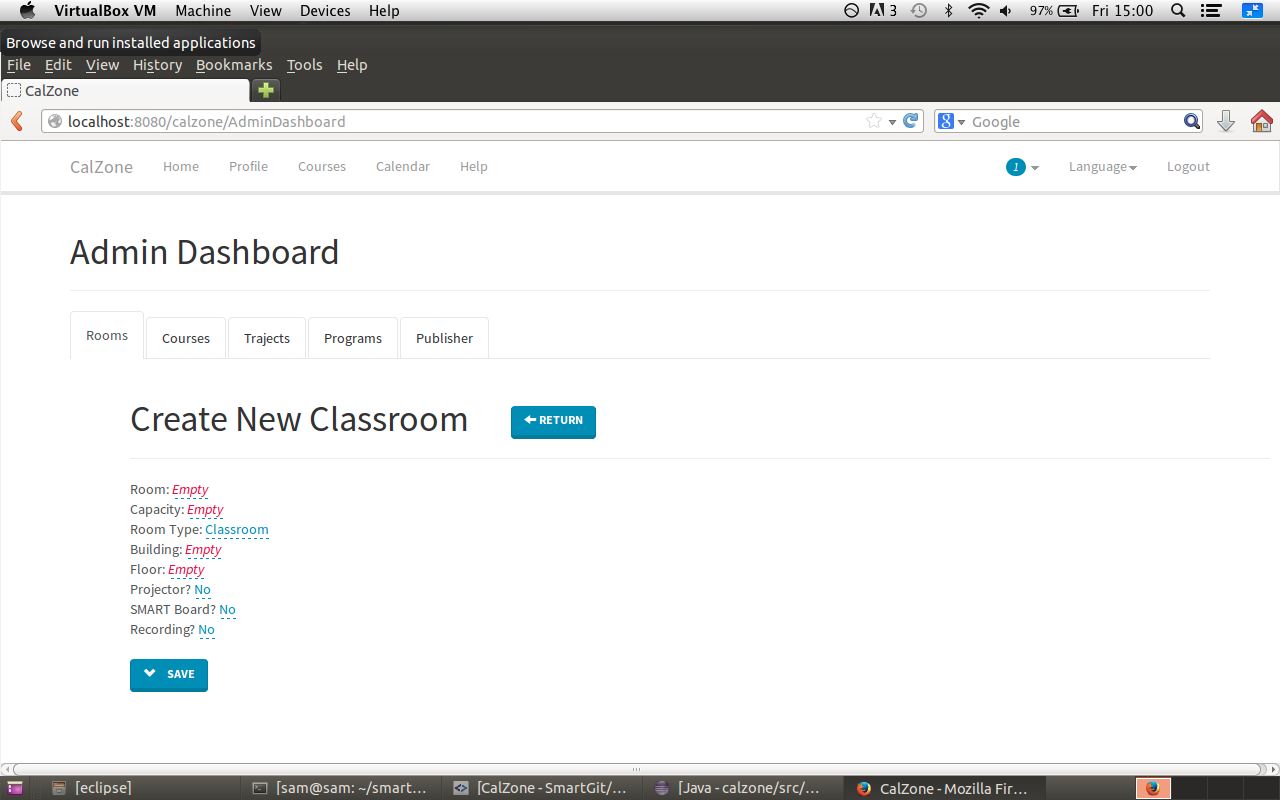
\includegraphics[scale=0.4]{img/CalzoneAdminNewClassroom}}
\label{fig:CalZone New Classroom}
\end{figure}
\end{center}

%Lokaal detailformulier verwijderen
\subsubsection{Lokaal detailformulier verwijderen}        
\noindent\begin{table}[H]
            \begin{tabular}{l | p{10cm}}
                \textbf{ID:} & FR3.2 \\ \hline
                \textbf{TITEL:} & 3. Lokaal detailformulier verwijderen\\ \hline
                \textbf{PRIORITEIT:} &  Hoog \\ \hline
                \textbf{PREREQUISITIES:} & \\ \hline
                \textbf{TOEGANG:} & Programmabeheerder \\ \hline
                \textbf{BESCHRIJVING:} & De Programmabeheerder moet in staat zijn lokalen te verwijderen (In het geval dat deze niet meer in gebruik worden genomen).\\ 
            \end{tabular}\\
            \caption{FR3.2 - Lokaal detailformulier verwijderen}
            \label{tab:FR3.2- Lokaal detailformulier verwijderen}
        \end{table}
        
\textbf{Stappenplan:}       
\begin{enumerate}
\item De programmabeheerder ziet zijn beginscherm op zijn webbrowser. Hier ziet hij de optie "lokalen".
\item De programmabeheerder klikt hierop en wordt doorverwezen naar een nieuwe pagina waar hij de optie ziet om lokalen te verwijderen (zie figuur \ref{fig:CalZone Remove Course}).
\item De programmabeheerder klikt op de knop en krijgt een melding met de vraag of hij zeker is of hij dit lokaal wil verwijderen.
\item De programmabeheerder klikt op \"ja\" en voert de verwijdering hierdoor permanent door.
\end{enumerate}      

\begin{center}
\begin{figure}[H]
\caption{CalZone Remove Course}
\centerline{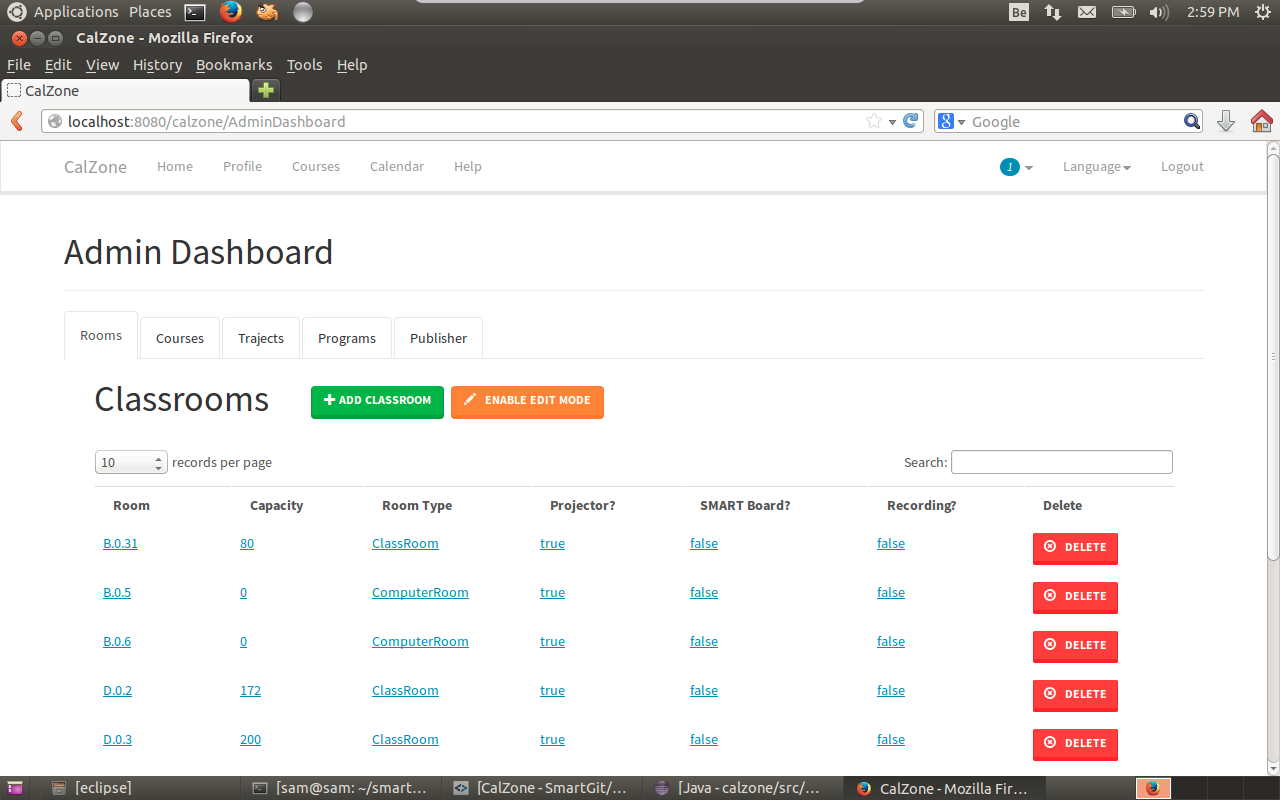
\includegraphics[scale=0.4]{img/CalzoneAdminClassrooms}}
\label{fig:CalZone Remove Course}
\end{figure}
\end{center}

%Lokaal detailformulier aanpassen
\subsubsection{Lokaal detailformulier aanpassen} 
\noindent\begin{table}[H]
            \begin{tabular}{l | p{10cm}}
                \textbf{ID:} & FR3.3 \\ \hline
                \textbf{TITEL:} & Lokaal detailformulier aanpassen\\ \hline
                \textbf{PRIORITEIT:} &  Medium \\ \hline
                \textbf{PREREQUISITIES:} & \\ \hline
                \textbf{TOEGANG:} & Programmabeheerder \\ \hline
                \textbf{BESCHRIJVING:} & Mocht er nood zijn aan het aanpassen van een lokaal detailformulier, moet de programmabeheerder de optie hebben om dit te doen.\\ 
            \end{tabular}\\
            \caption{FR3.3 - Lokaal detail formulier aanpassen}
            \label{tab:FR3.3 - Lokaal detailformulier aanpassen}
        \end{table}
        
\textbf{Stappenplan:}
\begin{enumerate}
\item De programmabeheerder ziet zijn beginscherm op zijn webbrowser. Hier ziet hij de optie "lokalen".
\item De programmabeheerder klikt hierop en wordt doorverwezen naar een nieuwe pagina waar hij de optie ziet om lokalen te verwijderen.
\item De programmabeheerder klikt op deze optie en wordt doorverwezen naar een nieuwe pagina met 3 lijsten, respectievelijk voor de gebouwen, verdiepingen en de lokalen.
\item De programmameerbeheerder selecteert telkens de gewenste optie in de lijsten en ziet een knop met de naam "lokaal wijzigen".
\item De programmabeheerder klikt op de knop en krijgt het detailformulier van het lokaal te zien.
\item De programmabeheerder past de nodige gegevens aan en ziet een knop met de naam "Wijzigingen opslaan".
\item De programmabeheerder klikt op deze knop en voert hierdoor de wijzigingen permanent door.
\end{enumerate}

\begin{center}
\begin{figure}[H]
\caption{CalZone Edit Course}
\centerline{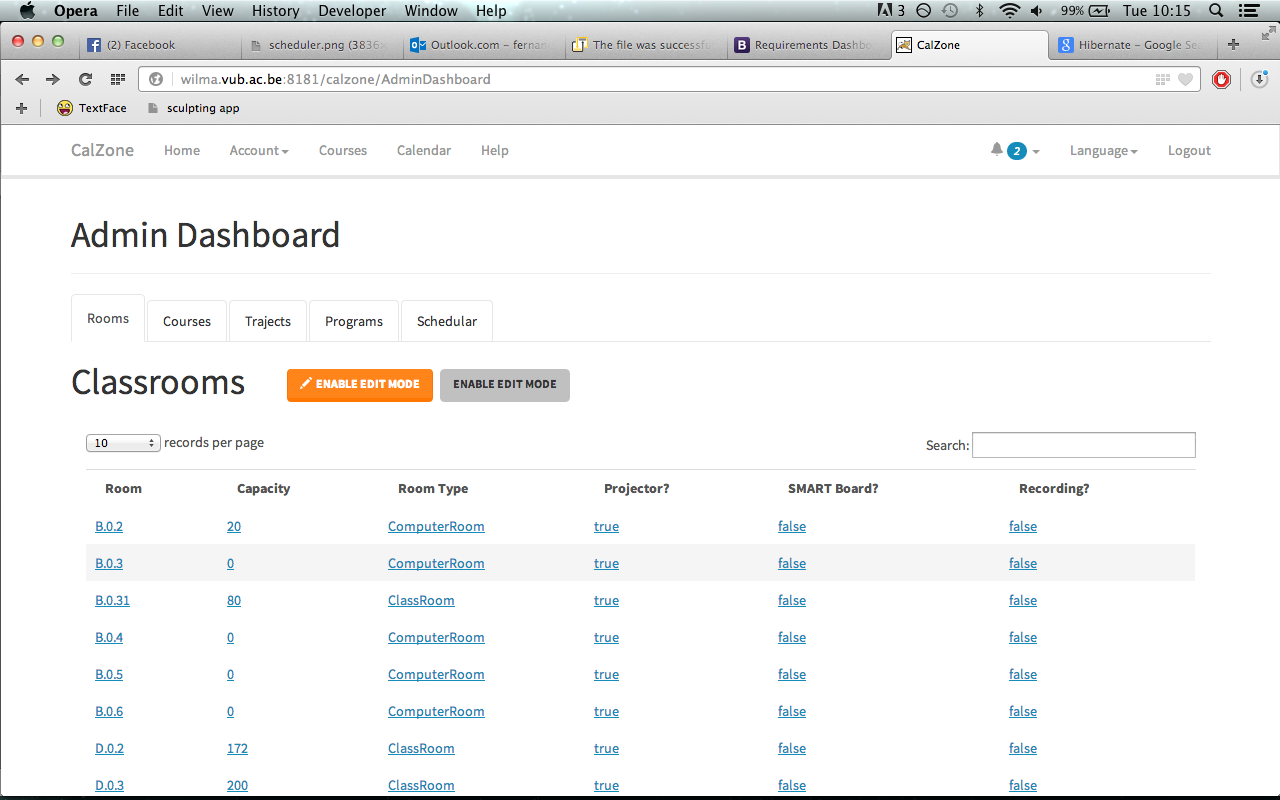
\includegraphics[scale=0.4]{img/CalzoneAdminClassroomsEdit}}
\label{fig:CalZone Edit Course}
\end{figure}
\end{center}


%GPS locatie van lokaal
\subsubsection{GPS Locatie} 
\noindent\begin{table}[H]
            \begin{tabular}{l | p{10cm}}
                \textbf{ID:} & FR3.4 \\ \hline
                \textbf{TITEL:} & GPS Locatie\\ \hline
                \textbf{PRIORITEIT:} &  Laag \\ \hline
                \textbf{PREREQUISITIES:} & \\ \hline
                \textbf{TOEGANG:} & Aangemelde Gebruiker \\ \hline
                \textbf{BESCHRIJVING:} & Elk lokaal moet voorzien zijn van een GPS locatie die opgevraagd kan worden.\\ 
            \end{tabular}\\
            \caption{FR3.4 - GPS Locatie}
            \label{tab:FR3.4 - GPS Locatie}
        \end{table}
\clearpage